\documentclass{article}
\renewcommand\labelenumi{(\theenumi)}
% if you need to pass options to natbib, use, e.g.:
% \PassOptionsToPackage{numbers, compress}{natbib}
% before loading nips_2016
%
% to avoid loading the natbib package, add option nonatbib:
% \usepackage[nonatbib]{nips_2016}

\usepackage{nips_2016}

% to compile a camera-ready version, add the [final] option, e.g.:
% \usepackage[final]{nips_2016}

\usepackage[utf8]{inputenc} % allow utf-8 input
\usepackage[T1]{fontenc}    % use 8-bit T1 fonts
\usepackage{hyperref}       % hyperlinks
\usepackage{url}            % simple URL typesetting
\usepackage{booktabs}       % professional-quality tables
\usepackage{amsfonts}       % blackboard math symbols
\usepackage{nicefrac}       % compact symbols for 1/2, etc.
\usepackage{microtype}      % microtypography
\usepackage{amsmath}
\usepackage{graphicx}

\title{Discovering visual phenomena at multiple scales using the hierarchical Latent Dirichlet Allocation}

% The \author macro works with any number of authors. There are two
% commands used to separate the names and addresses of multiple
% authors: \And and \AND.
%
% Using \And between authors leaves it to LaTeX to determine where to
% break the lines. Using \AND forces a line break at that point. So,
% if LaTeX puts 3 of 4 authors names on the first line, and the last
% on the second line, try using \AND instead of \And before the third
% author name.

\author{
  Genevieve Flaspohler \thanks{Use footnote for providing further
    information about author (webpage, alternative
    address)---\emph{not} for acknowledging funding agencies.} \\
  Department of Computer Science\\
  Cranberry-Lemon University\\
  Pittsburgh, PA 15213 \\
  \texttt{hippo@cs.cranberry-lemon.edu} \\
}

\begin{document}

\maketitle

\begin{abstract}
Marine robots operate in the most communication constrained environments on earth. These challenging conditions require marine robots to display high levels of autonomy. Semantic understanding is an essential precursor to meaningful autonomy. Throughout the scientific community, hierarchical trees appear as a powerful and concise manner of representing complex semantic knowledge. In this work, I apply the Bayesian nonparametric hierarchical Latent Dirichlet Allocation (hLDA) model to data collected by the Jaguar AUV off the Hannibal Sea Mount, Panama to discover hierarchical associations among the observed visual data. 
\end{abstract}

\section{The Hierarchical Latent Dirichlet Allocation model}
  The Hierarchical Latent Dirichlet Allocation (hLDA) model was introduced by \citet{Blei2010}. Compared to a flat LDA model, hLDA is able to model a richer class of hierarchical relationships among topics, while maintaining the nonparametric properties of HDP topic models. The foundation of this model is the nested Chinese Restaurant Process (nCRP). The nCRP is nonparametric prior over infinitely deep, infinitely branching trees. Each node $k$ in this infinite tree represents a topic $\beta_k$, and each document is defined by a path down the tree $\mathbf{c}_d$. Each path starts with the most general topic at the tree root. Therefore, each document shares this most general topic. The topics in the leaf nodes will be shared by a much more restricted subset of documents, and represent more specific semantic constructs. The full generative model and graphical representation for hLDA presented in \citet{Blei2010} are reproduced in the Appendix.

\subsection{Gibbs Sampling Inference}
\citet{Blei2010} introduces a collapsed Gibbs sampler to do inference in the hLDA model. The topic parameters $\beta_k$ and the per-document topic proportions $\theta_d$, are integrated out to speed up the chain's convergence. For each iteration of the sampler, the per-document paths $\mathbf{c}_d$ and the per-word level allocations to topics in those paths $z_{d,n}$ are sampled from the equations reproduced in the Appendix. 

\subsection{Code implementation}
\citet{Blei2010} provides a C implementation of the hLDA model. The code is flexible enough to work directly on appropriately discretized image data from a marine robotic mission. The documentation for this code is fairly poor, so I have spent a good amount of time understanding how to run the code and interpret and visualize the output. I then tested the implementation on downloaded articles from the Associated Press and coded my own generative model for hLDA in order to test Blei's code on simulated data. The results of these experiments are discussed in Section \ref{sec:exp}.

\section{Data experiments}
\label{sec:exp}
\subsection{Associated Press abstracts}
I applied the hLDA code to discover hierarchical structure in Associated Press news articles. In \citet{Blei2010}, results are presented for the full dataset of 2246 documents. However, after running the code for three days, it had only completed 1000 of the ten thousand epochs. Instead, I tested the algorithm on a 500 document subset of these articles. The highest likelihood recovered hierarchical topic structure is visualized in Figure \ref{fig:sim}.

\begin{figure}[h]
  \centering
    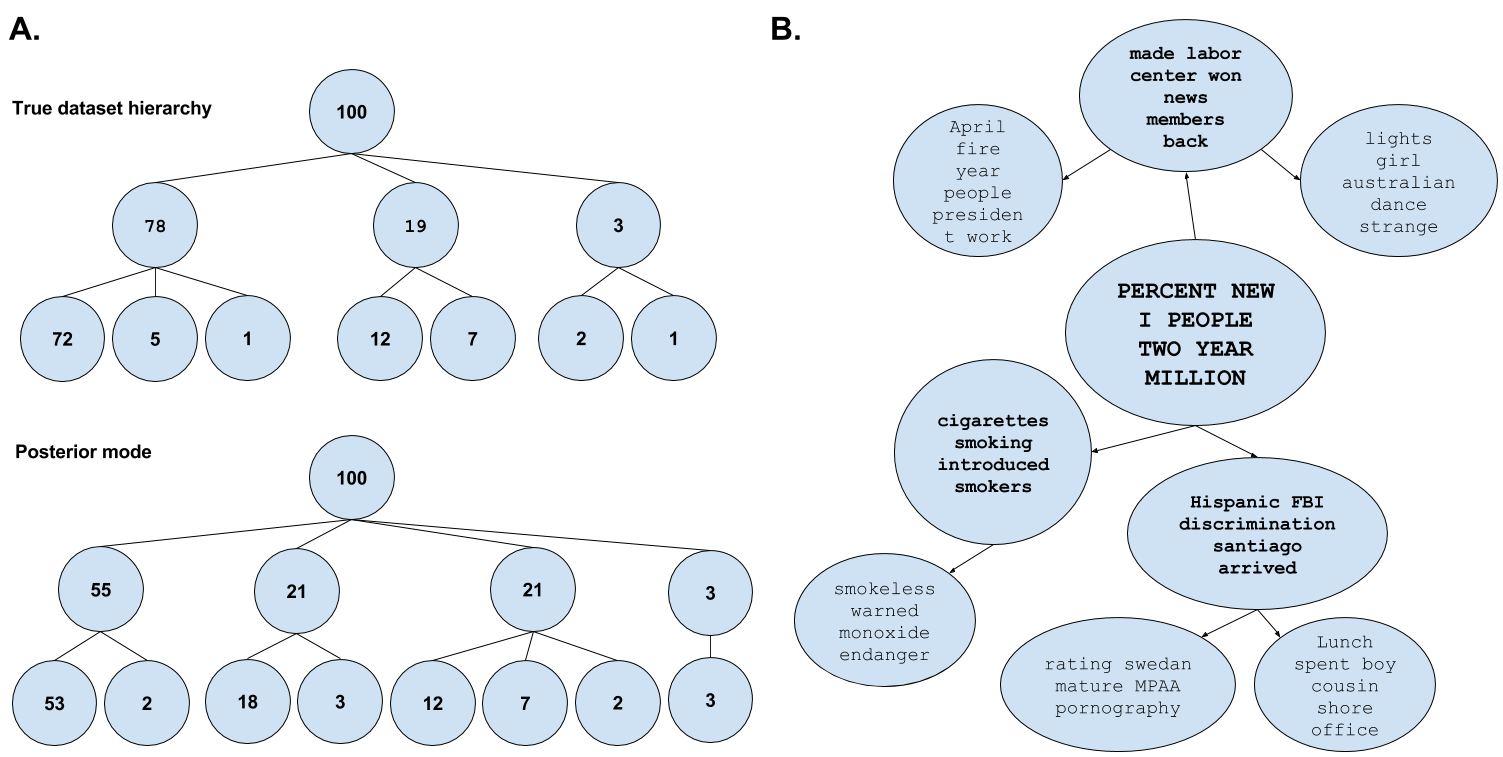
\includegraphics[scale=0.25]{sim}
  \caption{The results of running hLDA posterior inference on 100 simulated documents and 500 Associated Press news articles. A) The performance of the algorithm on 100 simulated documents, 250 words each. Each node in the tree represents a topic, and the number of documents containing that document is shown directly on the node. The true topic hierarchy (top) was always smaller than the trees recovered by posterior inference (bottom) .}
  \label{fig:sim}
\end{figure}

\subsection{Simulated generative model}
\citet{Blei2010} also presents the results of using the described inference procedure to recover model parameters on data simulated from the generative model. With hyperparameter settings $\eta = 0.005$ and $\gamma = 1$, they generate 100 documents of 250 words each. In the simulations, the stick breaking procedure used to determined the depth of the tree was truncated after three levels; arbitrary branching factor was allowed. To reproduce the results, I implemented the generative model described and ran it with the same hyperparameter settings \footnote{https://github.com/geflaspohler/hlda/tree/master/generative}. After 10,000 rounds of Gibbs sampling, the tree that produced the highest log-likelihood (the "mode") was chosen as the true tree, as described in the paper. However, unlike the results presented in the paper, the provided hLDA code does not seem to recover the true tree structure well, even after five cross-validation runs. An example of the true simulated tree structure and the structure discovered using inference is shown in Figure \ref{fig:sim}.

\section{Remaining action items}
Despite the algorithm's failure on simulated data, it appears to recover a reasonable topic hierarchy from the Associated Press articles. It is possible that there is a mistake or misinterpretation in my simulated model, or that the authors in \citet{Blei2010} used some other methods not described in their paper to infer the simulated models with such high accuracy. I will continue to adjust the simulation, but meanwhile I will move ahead to applying the model on image data.

In \citet{Sivic}, the hLDA model is applied to images to recover a semantic hierarchy among simple classes of objects (e.g. cars from several vantage points, stoplights, computer screens). I will follow the word-extraction process introduced in this paper (SIFT features at multiple scales) to convert my image data into discrete words, which can then be fed directly into the hLDA model. One potential issue raised by \citet{Sivic} is that initialization has a large impact on the optimality of the tree structure recovered. They use a heuristic that assigns a good initial guess to the level of abstraction of visual words using properties of the image. Given time, I will attempt to also explore the effect of initialization of the recovered model. 

\bibliographystyle{unsrtnat}
\bibliography{hlda}

\newpage
\section*{Appendix}

\subsection*{Generative model}
The Hierarchical Latenet Dirichlet Allocation (hLDA) model defines the following generative process for documents
%\begin{enumerate}{(1)}
\begin{enumerate}
  \item For each table $ k \in \cal{T}$ in the infinite tree,
  \begin{enumerate}
    \item Draw a topic $\beta_k \sim \text{Dirichlet}(\eta)$
  \end{enumerate}
  \item For each document, $d \in \{1, 2, \dots , D\}$
    \begin{enumerate}
      \item Draw a path through the tree, $\mathbf{c}_d \sim \text{nCRP}(\gamma)$.
      \item Draw a distribution over levels in the tree, $\theta_d | \{m, \pi\} \sim \text{GEM}(m, \pi)$
      \item For each word,
        \begin{enumerate}
          \item Choose level $Z_{d,n} | \theta_d \sim \text{Discrete}(\theta_d)$
          \item Choose word $W_{d,n} | \{ z_{d,n}, \mathbf{c}_d, \beta \} \sim \text{Discrete}(\beta_{\mathbf{c}_d}[z_{d,n}])$, which is parameterized by the topic in position $z_{d,n}$ on the path $\mathbf{c}_d$.
        \end{enumerate}
    \end{enumerate}
\end{enumerate}

\subsection*{Gibbs Sampling Updates}
The Gibbs sampler described in \citet{Blei2010} itertively samples the per-document path assignment variables and the per-word level assignment variables. 
\begin{enumerate}
  \item For each document $d \in \{ 1, \dots , D\}$
  \begin{enumerate}
    \item Randomly draw $\mathbf{c}_d^{(t+1)}$ from Eq. \citet{eq1}
    \item Randomly draw $z_{n,d}^{(t+1)}$ from Eq. \citet{eq2} for each word, $n \in \{1, \dots , N_d\}$
  \end{enumerate}
\end{enumerate}

\subsubsection*{Sampling Level Allocations}
The posterior level assignment for word $n$ in document $d$ can be written as:
\begin{equation}
\begin{split}
  P(z_{d,n} | \mathbf{z}_{-(d,n)}, \mathbf{c}, \mathbf{w}, m, \pi, \eta) & \propto P(z_{d,n} | \mathbf{z}_{d, -n}, m, \pi) P(w_{d,n} | \mathbf{z}, \mathbf{c}, \mathbf{w}_{-(d,n)}, \eta) \\
P(z_{d,n} | \mathbf{z}_{d, -n}, m, \pi) & = \frac{m\pi + \#[\mathbf{z}_{d, -n} = k]}{\pi + \#[\mathbf{z}_{d, -n} \geq k]} \prod_{j = 1}^{k-1} \frac{(1-m)\pi + \#[\mathbf{z}_{d, -n} > j]}{\pi + \#[\mathbf{z}_{d, -n} \geq j]} \\
  P(w_{d,n} | \mathbf{z}, \mathbf{c}, \mathbf{w}_{-(d,n)}, \eta) & \propto \#[\mathbf{z}_{-(d,n)} = z_{d,n}, \mathbf{c}_{z_{d,n}} = c_{d,z_{d,n}}, \mathbf{w}_{-(d,n)} = w_{d,n}] + 
  \eta\\
\end{split}
\end{equation}

\subsubsection*{Sampling Paths}
The posterior level assignment for word $n$ in document $d$ can be written as:
\begin{equation}
\begin{split}
  P(\mathbf{c}_d | \mathbf{w}, \mathbf{c}_{-d}, \mathbf{z}, \eta, \gamma) & \propto P(\mathbf{c}_{d} | \mathbf{c}_{-d}, \gamma) P(\mathbf{w}_{d} | \mathbf{c}, \mathbf{w}_{-d}, \mathbf{z},\eta) \\
  P(\mathbf{c}_{d} | \mathbf{c}_{-d}, \gamma)  & \text{is given by the nCRP prior} \\
  P(\mathbf{w}_{d} | \mathbf{c}, \mathbf{w}_{-d}, \mathbf{z},\eta) & \propto \frac{\prod_w \Gamma (\#[\mathbf{z} = l, \mathbf{c}_{l} = c_{d,l}, \mathbf{w} = w] + \eta}{\Gamma (\sum_w \#[\mathbf{z} = l, \mathbf{c}_{l} = c_{d,l}, \mathbf{w} = w] + V\eta)}\\
\end{split}
\end{equation}

\end{document}
